\documentclass[varwidth=true, border=2pt]{standalone}
\usepackage{tikz}
\usepackage{pgfplots}
\usepackage{amsmath,amssymb}

\begin{document}
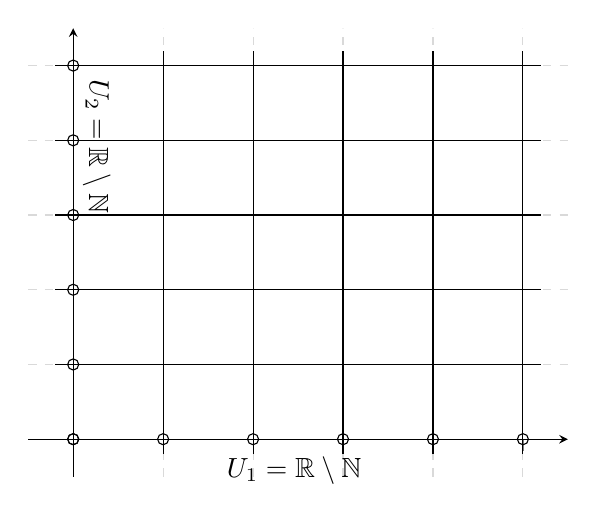
\begin{tikzpicture}
    \begin{axis}[
        axis x line=middle,
        axis y line=middle,
        grid = major,
        grid style={dashed, gray!30},
        xmin= 0,     % start the diagram at this x-coordinate
        xmax= 5,    % end   the diagram at this x-coordinate
        ymin= 0,     % start the diagram at this y-coordinate
        ymax= 5,   % end   the diagram at this y-coordinate
        xtick={-1,0,1,2,3,4,5},
        ytick={-1,0,1,2,3,4,5},
        xlabel={$U_1 = \mathbb{R} \setminus \mathbb{N}$},
        xlabel style={xshift=-2.5cm,yshift=-0.7cm},
        ylabel={$U_2 = \mathbb{R} \setminus \mathbb{N}$},
        ylabel style={rotate=-90, xshift=1.5cm},
        xticklabels={,,},
        yticklabels={,,},
        tick align=outside,
        enlargelimits=true]


        % Draw solid square
        \addplot[mark=o] coordinates {(0,0) (1,0) (2,0) (3,0) (4,0) (5,0)};
        \addplot[mark=o] coordinates {(0,0) (0,1) (0,2) (0,3) (0,4) (0,5)};

        \foreach \i in {0,1,2,3,4,5} {
            \addplot[mark=none] coordinates {(-0.2,\i) (5.2,\i)};
            \addplot[mark=none] coordinates {(\i,-0.2) (\i,5.2)};
        }
        \addplot[mark=none] coordinates {(0,2) (5,2)};
    \end{axis} 
\end{tikzpicture}
\end{document}
